\chapter{Database Design}
\section{Data Dictionary}
\begin{table}[h]
\begin{tabular}[center]{|l|l|l|l|l|}
  \hline
  \multicolumn{5}{|c|}{User} \\
  \hline
  Fields & Data Type & Null/Not Null & Key & Default \\
  \hline
  name & varchar(50) & Not Null & - & - \\
  surnname & varchar(50) & Not Null & - & - \\
  email & varchar(50) & Not Null & PRI & - \\
  password & varchar(50) & Not Null & - & - \\
  avatar & varchar(50) & Not Null & - & - \\
  \hline
\end{tabular}
\caption{\label{tab:table-name}Data Dictionary for User.}
\end{table}

\vspace{10 mm}

\begin{table}[h]
\begin{tabular}[center]{|l|l|l|l|l|}
  \hline
  \multicolumn{5}{|c|}{Board} \\
  \hline
  Fields & Data Type & Null/Not Null & Key & Default \\
  \hline
  title & varchar(50) & Not Null & PRI & - \\
  members & varchar(50) & Not Null & - & - \\
  list & varchar(50) & Not Null & - & - \\
  activity & varchar(50) & Not Null & - & - \\
  isImage & boolean & Not Null & - & - \\
  background image link & varchar(50) & Not Null & - & - \\
  \hline
\end{tabular}
\caption{\label{tab:table-name}Data Dictionary for Board.}
\end{table}

\vspace{10 mm}

\begin{table}[h]
\begin{tabular}[center]{|l|l|l|l|l|}
  \hline
  \multicolumn{5}{|c|}{List} \\
  \hline
  Fields & Data Type & Null/Not Null & Key & Default \\
  \hline
  owner & varchar(50) & Not Null & - & - \\
  title & varchar(50) & Not Null & - & - \\
  \hline
\end{tabular}
\caption{\label{tab:table-name}Data Dictionary for List.}
\end{table}

\vspace{10 mm}

\begin{table}[h]
\begin{tabular}[center]{|l|l|l|l|l|}
  \hline
  \multicolumn{5}{|c|}{Card} \\
  \hline
  Fields & Data Type & Null/Not Null & Key & Default \\
  \hline
  name & varchar(50) & Not Null & - & - \\
  title & varchar(50) & Not Null & - & - \\
  checklist & varchar(50) & Not Null & - & - \\
  description & varchar(50) & Not Null & - & - \\
  labels & varchar(50) & Not Null & - & - \\
  %members & varchar(50) & Not Null & - & - \\
  date & date & Not Null & - & - \\
  attachments & varchar(50) & Not Null & - & - \\
  activities & varchar(50) & Not Null & - & - \\
  %owner & varchar(50) & Not Null & - & - \\
  %cover & varchar(50) & Not Null & - & - \\
  \hline
\end{tabular}
\caption{\label{tab:table-name}Data Dictionary for Card.}
\end{table}
\vspace{10 mm}

\section{ER Diagrams}
\begin{figure}[h]
    \centering
    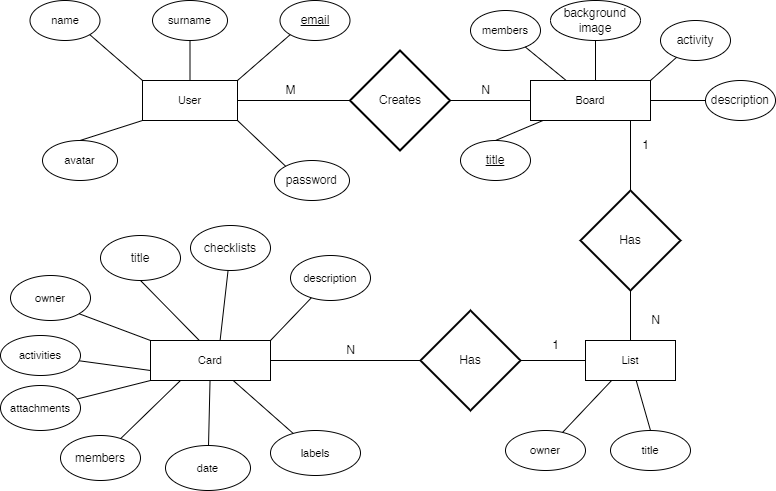
\includegraphics[width = 1.1\textwidth]{ER Diagram.drawio.png}\\[0.1in]
    \caption{ER Diagram}
    \label{fig:my_label}
\end{figure}
Include ER diagrams here and explain them
briefly



